\documentclass[oneside,11pt]{homework}
\usepackage{mathrsfs}
\usepackage{graphicx}
% \usepackage{pythonhighlight}
\usepackage{bm}
\usepackage{multicol}
\usepackage{float}
\usepackage{textcomp}
\usepackage{graphicx}

\setlength{\parindent}{0pt}
\setlength{\parskip}{0.5\baselineskip}

\coursename{GR5291 Advanced Data Analysis (Spring 2018)} % DON'T CHANGE THIS

\studnamea{Mingyu Jiao - mj2823}
\studnameb{Fan Yang - fy2232}
\studnamec{Qianhui Sun - qs2179}

\begin{document}
\maketitle

\section{}

\section*{1 Summary}

The goal of this project is to study which factors influence the number of serious crimes per county. The analysis shows that \textit{Percent of population aged 18-34}, \textit{Percent below poverty level}, \textit{Per capita income}, \textit{Percent of hospital beds}, \textit{Population density} and \textit{Region} are significant factors. Although \textit{Region} is important in the analysis, there is nothing can be done to improve this factor. While the other factors all have a positive relationship with \textit{crime rate}. Specifically, the results show that the higher level of these factors, the more likely for this county to have serious crime rate.\par
Based on the analysis, our advice for reducing the number serious crimes in their county is from three aspects: medical, population and salary. In other words, increasing the minimal salary, improving medical support and controling population density.

\section*{2 Introduction}
\subsection*{2.1 Description of the data}
The data we use is the county demographic information (CDI) data set from \textit{Applied Linear Statistical Models, 5th edition, by Kutner, Nachtsheim, Neter, and Li., Appendix C2.} This data set provides selected county demographic information for 440 of the most populous counties in the United States. Each line of the data set has an identification number with a county name and state abbreviation and provides information on 14 variables for a single county. Counties with missing data were deleted from the data set.\par

As the population differ from county to county, accumulation number is not as persuasive as percentage. Therefore rescaling some variables is needed. For example, we divide \textit{Total population} by \textit{Land area}; divide \textit{Total serious crimes}, \textit{Number of active physicians}, \textit{Number of hospital beds} and \textit{Number of hospital beds} by \textit{Total population}. After that, in order to have the same scale, we reduce these variables by 10 times. Finally, all those data roughly fall into the range $[10, 500]$.

\subsection*{2.2 Value/Benefit of the project}
The purpose of this project is to find the cause of serious crime rate. So based on our findings, government can determine which factors influence the number of serious crimes and implement policies that will lead to the reduction of the number serious crimes in their county. Specifically, crime rate in Kings county (Brookly) is in top level among all counties. Officials is thereby worried about their crime rate and help to reduce crime rate in Kings county is also purpose of this project.\par
Based on our project goal, we try to dig out the most significant factors among all variables in the dataset. After rescaling, we set pool of factors include 12 variables and one of them is categorical variables which is \textit{Geographic region}. And rest of them are numerical variables. Then we try to find out the significant influential factors.

\subsection*{2.3 Initial data exploration}
The subset that we use in the analysis consists of 12 independent variables. \textit{Geographic region} is the only categorical variables which has four categories (1=NE, 2=NC, 3=S, 4=W). 23.41\% of the counties are NE; 24.55\% are NC; 34.54\% are S and 17.5\% are W. We first explore whether region matters for crime rate(crime rate here is percentage instead of accumulation number).\par
\begin{figure}[H]
\centering
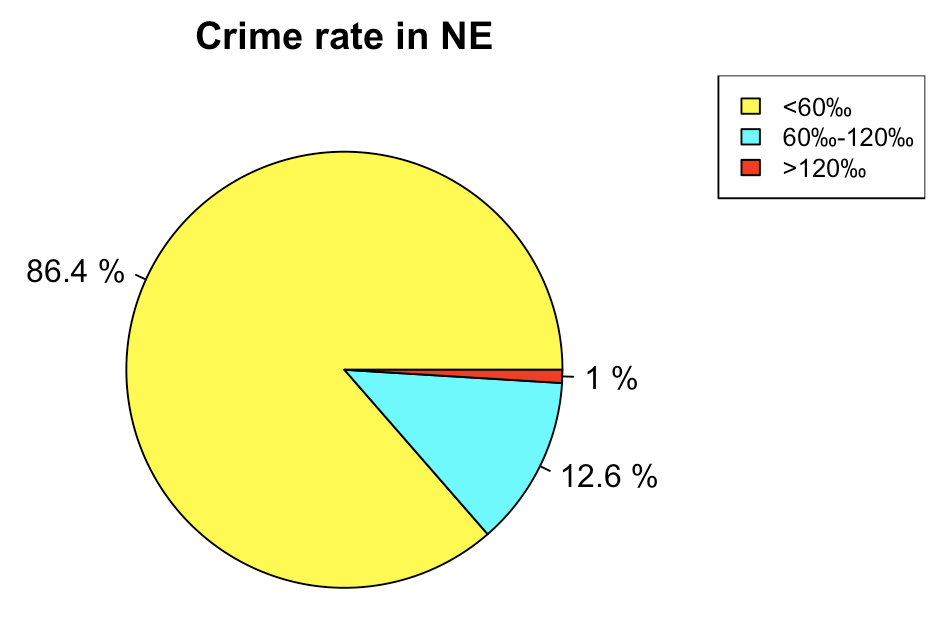
\includegraphics[scale=0.35]{NE.png}~~~~~
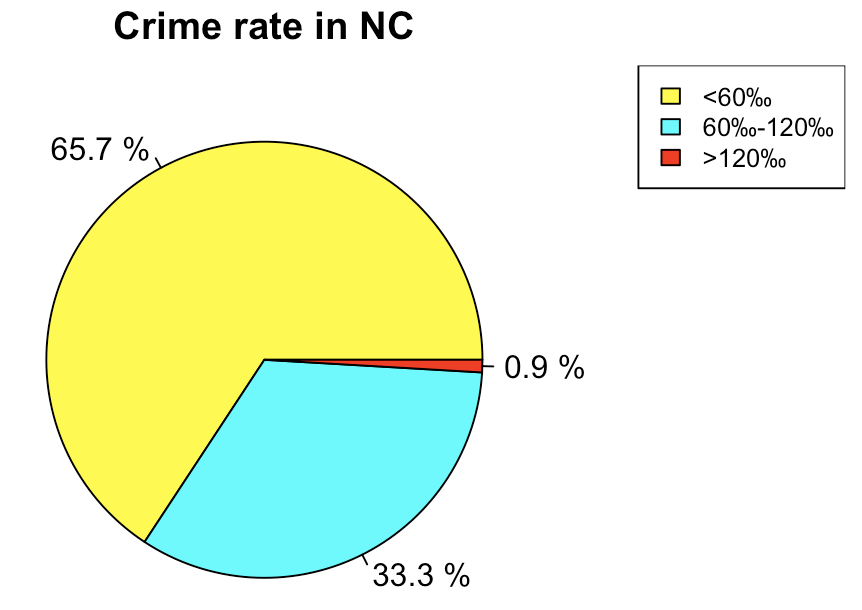
\includegraphics[scale=0.35]{NC.png}
\caption{Crime rate in region NE and NC} 
\end{figure}

\begin{figure}[H]
\centering
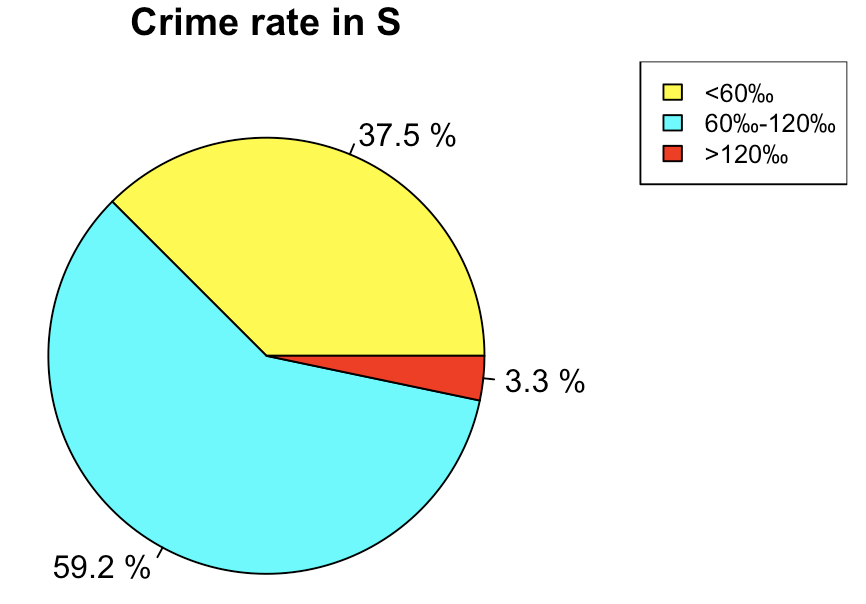
\includegraphics[scale=0.35]{S.png}~~~~~
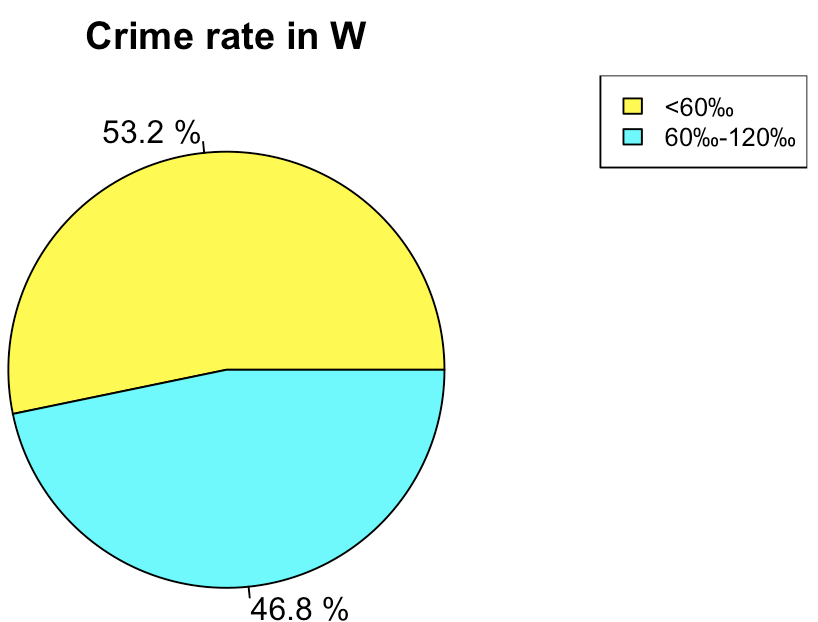
\includegraphics[scale=0.35]{W.png}
\caption{Crime rate in region S and W} 
\end{figure}
Of those counties in S, 20.4\% of them have crime rate above 90\textperthousand{}, while those counties in NE NC and W, less than 5\% have crime rate above 90\textperthousand{}. In the view of plot, crime rate in different regions differ greatly and counties in S tend to have severe crime rate.\par
Besides \textit{Geographic region}, we also find that \textit{Population density} and \textit{Percent below poverty level} important to explain high crime rate. Here we highlight the Kings county to compare its \textit{Population density} and \textit{Percent below poverty level} with all other counties. This is reasonable since crime rate in Kings county is much higher among all.

\begin{figure}[htbp]
\centering
\begin{minipage}[t]{0.48\textwidth}
\centering
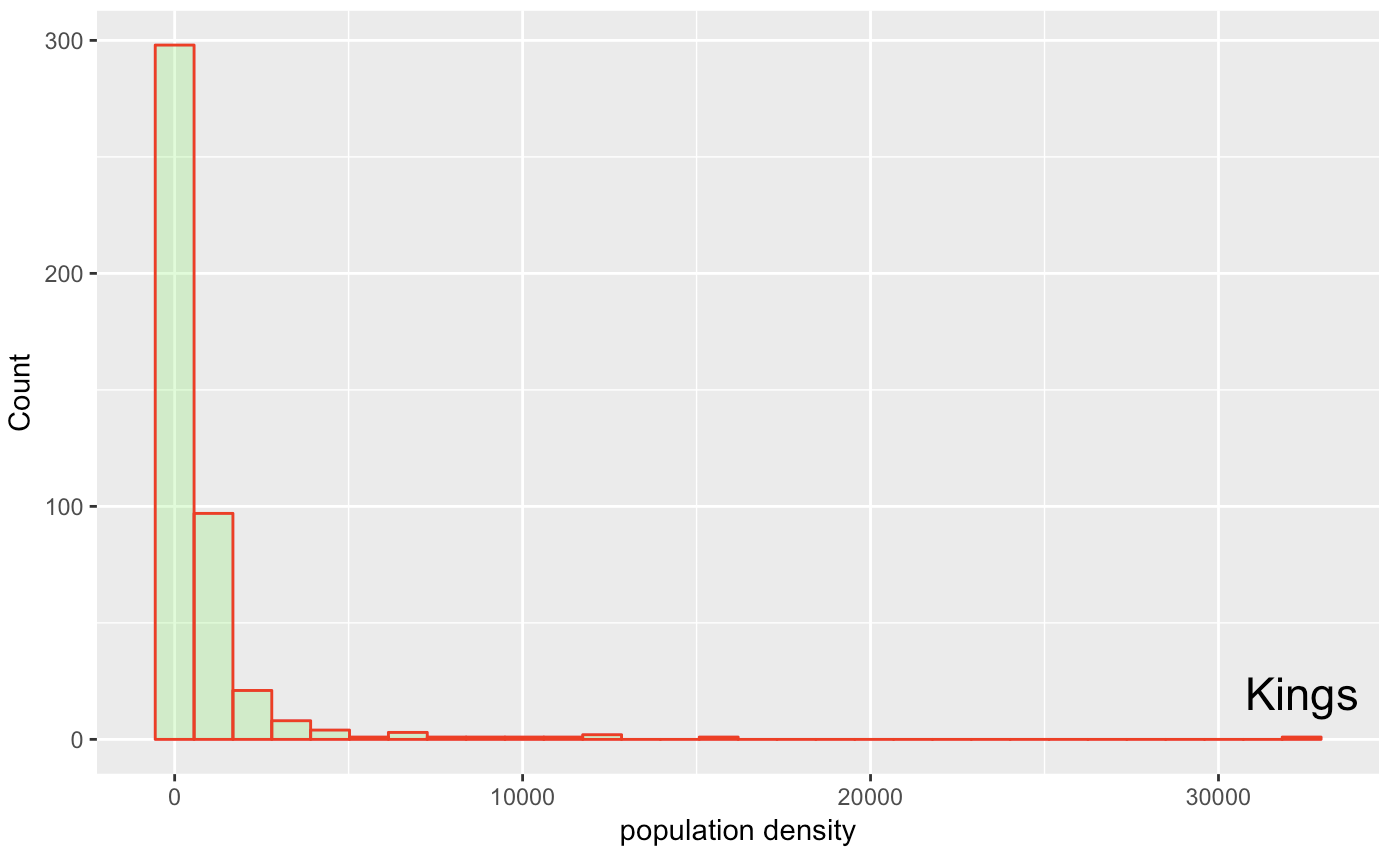
\includegraphics[scale=0.32]{density.png}
\caption{Population density histogram}
\end{minipage}
\begin{minipage}[t]{0.48\textwidth}
\centering
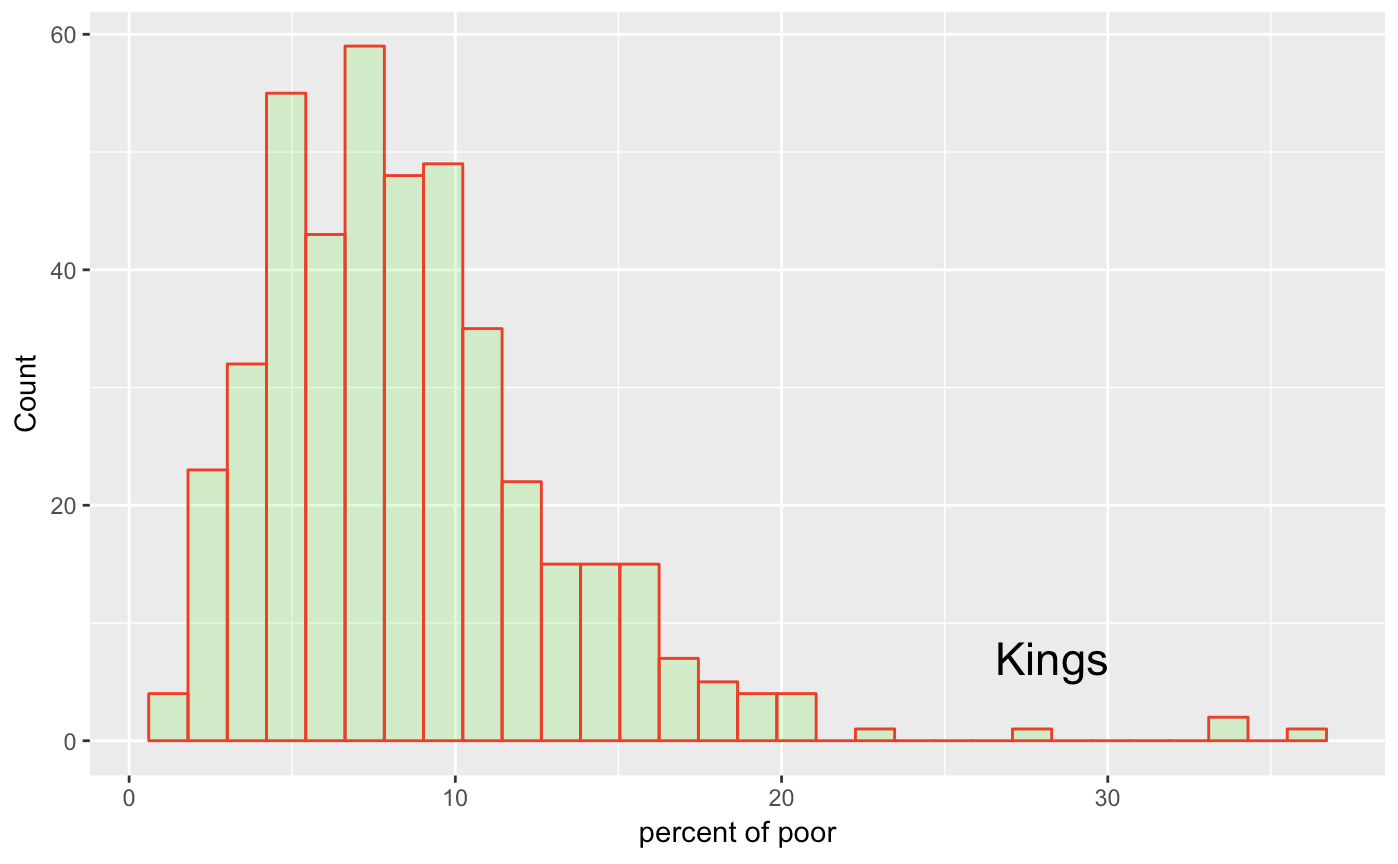
\includegraphics[scale=0.32]{poor.png}
\caption{Percent of poor histogram}
\end{minipage}
\end{figure}

The average population density is around 888 per square miles, while in Kings county, the population density is above 30000 per square miles, much higher than most of the counties. The average percent below
poverty level is around 9\%, while in Kings county, it is about 28\%, which is 2 times more than the average level.

\section*{3 Analysis and Results}
We use three models to to analyze this data: regular linear regression, poison regression and logistic regression. The results are slightly different in the three models but the significant factors which stand out in the three models are the same. The analysis shows that \textit{Percent of population aged 18-34}, \textit{Percent below poverty level}, \textit{Per capita income}, \textit{Percent of hospital beds}, \textit{Population density} and \textit{Region} are significant factors.

\subsection*{3.1 Linear Regression}

To analyze the influence factors of crime rate, the linear regression is the first choice. If the p-value of an independent variable is less than confidence level(0.05), we can say this variable has significant effects on crime rate generally.  We assume that those variables follow normal distribution and independent variables have linear relation with crime rate. \par

At first, we simply use the full linear regression model to analyze the data. Before fit model, we use Variance inflation factor(VIF) method to check the collinearity. The higher value of VIF, the more likely this variable is related with others. Therefore we drop the \textit{Percent bachelor’s degree} since it has high VIF(greater than 5).\par
\begin{figure}[H]
\centering
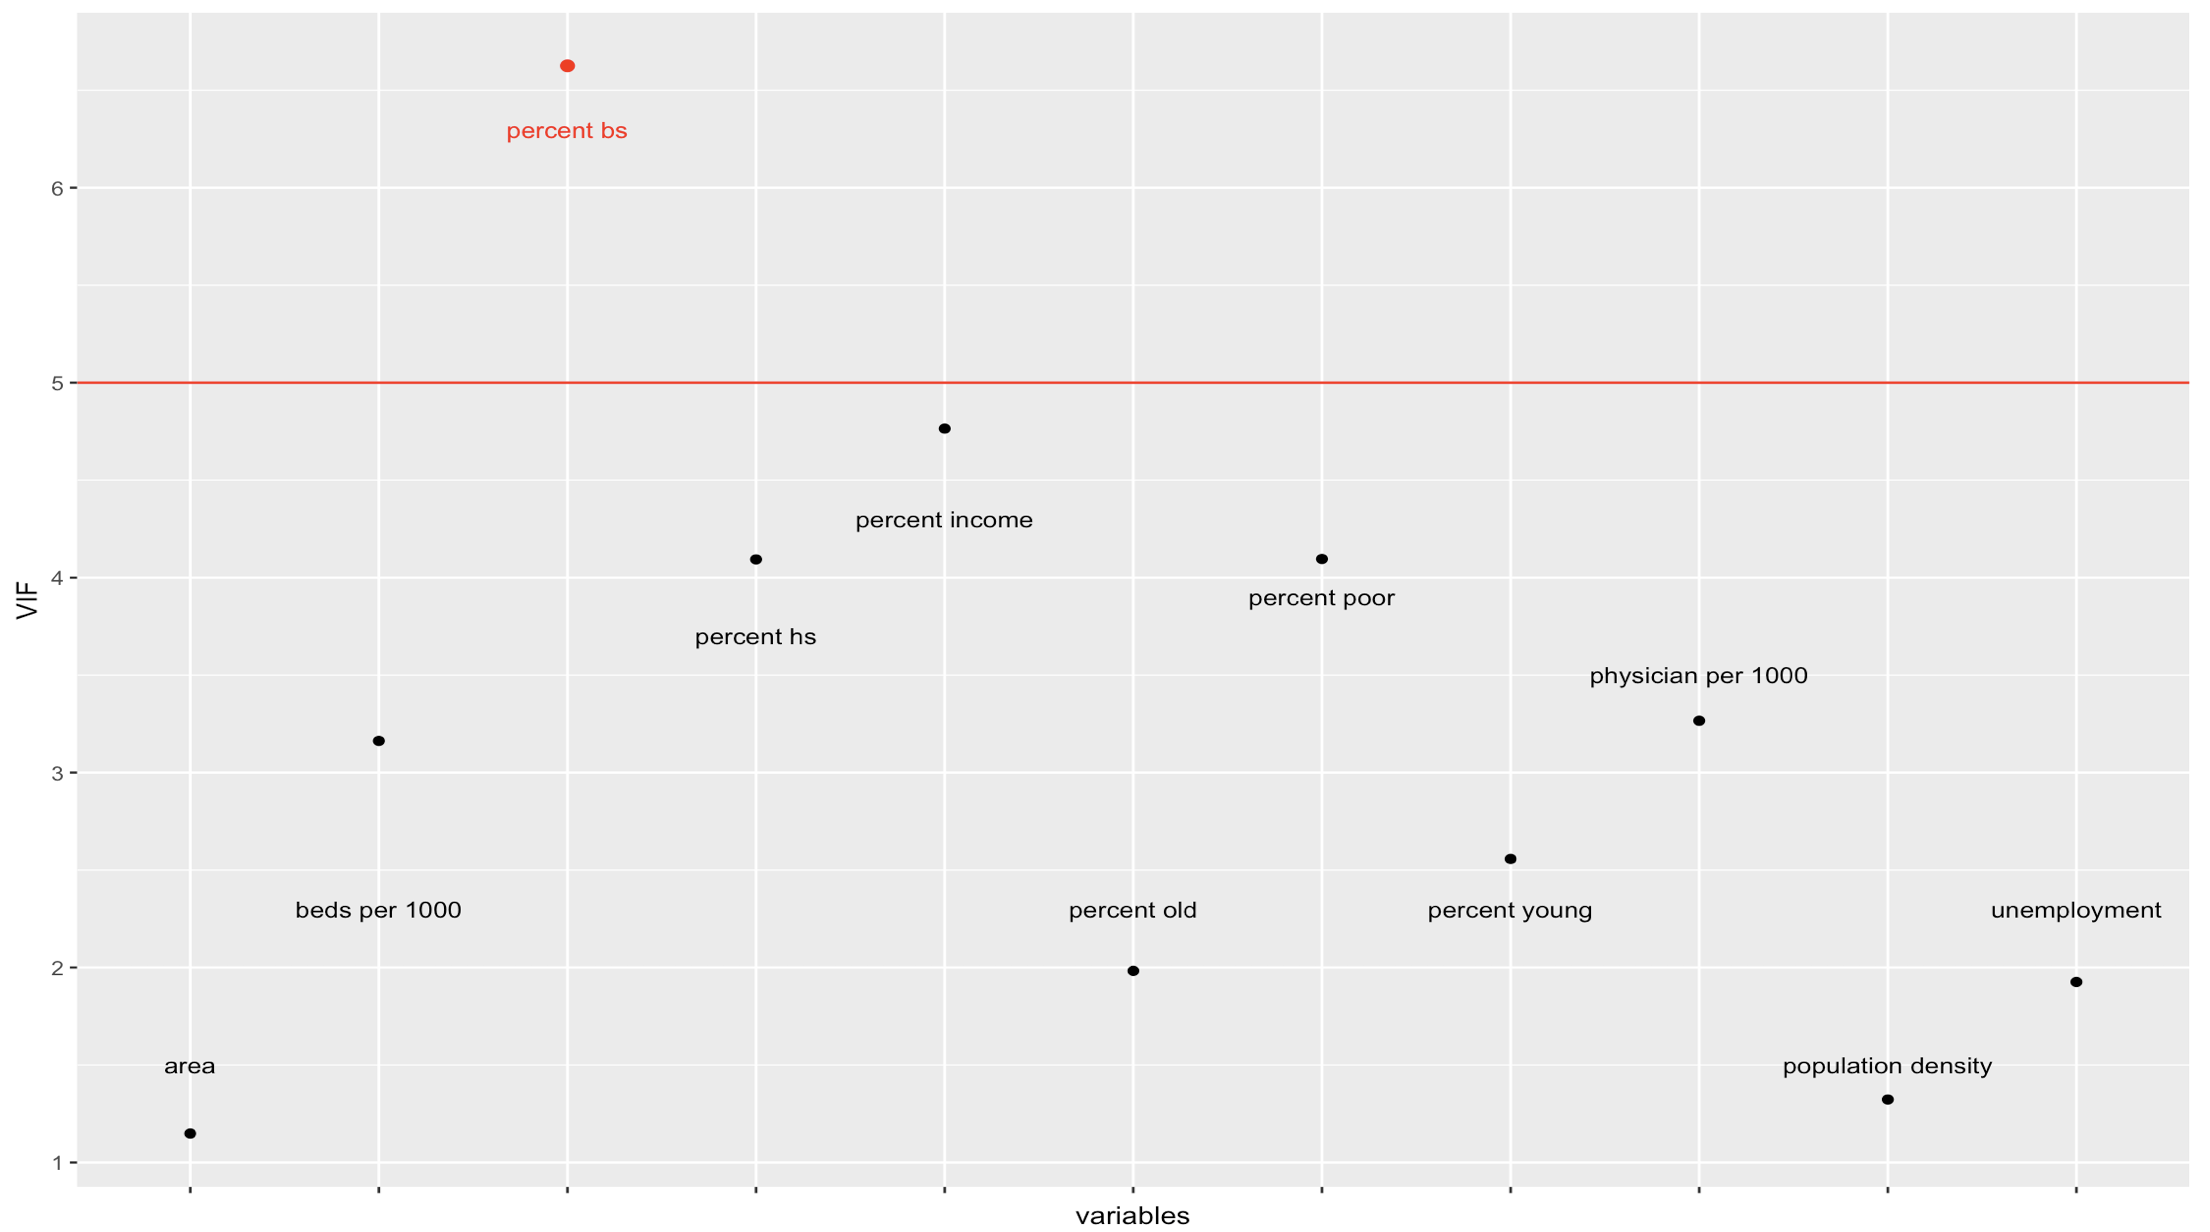
\includegraphics[scale=0.35]{VIF.png}
\caption{VIF plot} 
\end{figure}

Then we run the regression with the rest ten independent variables. In order to obtain a better model, we need to do variable selection. Use backward AIC to achieve this. The AIC for full model is 2577.49 and AIC for the best reduced model is 2570.99. And least AIC can be reached when drop \textit{percent of old}, \textit{percent of income}, \textit{unemployment}, \textit{area}. The regression result shows that under 0.05 confidence level, there are only 5 variables are significant. They are \textit{percent of young}, \textit{perc of poor}, \textit{percent of hospital beds}, \textit{geographic region}, \textit{population density}. So we can get the final model and the estimated coefficients are shown in Table 1.\par

\begin{table}[H]
\centering
\begin{tabular}{|c|c|c|c|c|c|c|}
\hline
\hline
\multicolumn{2}{|c|}{}&percent & percent  & percent & region & population\\
\multicolumn{2}{|c|}{}&young   & poor     & beds    &        & density  \\
\hline
\multicolumn{2}{|c|}{estimated coefficients} & 0.689 & 1.674& 2.60 & 9 & 0.0046\\
\hline
\hline
confidence&lower 2.5\% & 0.2713 & 1.1080& 1.5946 & 7.1987 & 0.0037\\
\cline{2-7}
interval&upper 97.5\% & 1.1068 & 2.2398& 3.5957 & 10.8158 & 0.0055\\
\hline
\end{tabular}
\caption{Estimated coefficient table}
\end{table}

From the analysis, we can get the interpretation of the parameter of the variable. Take perc.young as an example, if we increase the percent of population aged 18-34 by one, the crime rate per 1000 people will increase by about 0.689. And also we can get the confidence interval for those variables. Still take perc.young as an example, we are 95\% confident that a one unit increase in the percent of population aged 18-34 will increase on average the crime rate per 1000 people by a number between 0.271 and 1.107. \par


\subsection*{3.2 Poison Regression}
Poisson regression is used to model response variables that are counts. It tells you which explanatory variables have a statistically significant effect on the response variable. It’s best used for rare events, as these tend to follow a Poisson distribution. Poisson regression assumes the response variable has a Poisson distribution, and assumes the logarithm of its expected value can be modeled by a linear combination of unknown parameters. Poisson regression may also be appropriate for rate data, where the rate is a count of events divided by some measure of that unit's exposure. Thanks to the assumption, Poisson regression which could describe many real-world problems perfectly. So, we try this model to analyze this crime problem.\par

Before fit a Poisson regression, we use Pearson correlation to detect highly correlated variables. 

\begin{figure}[H]
\centering
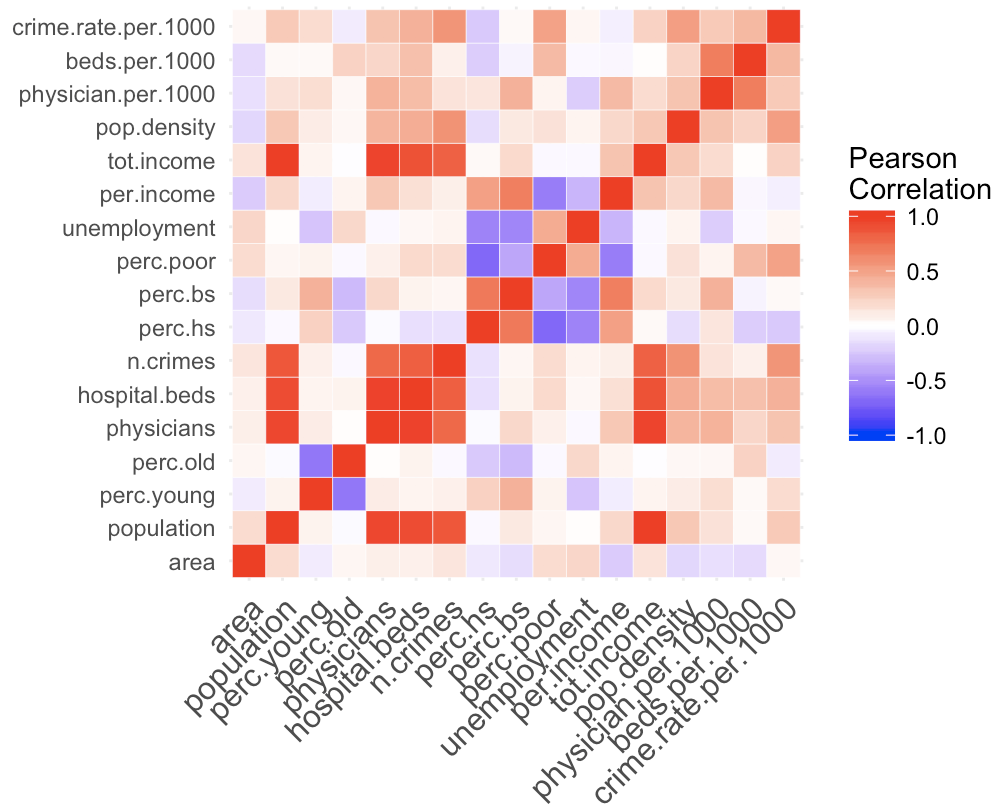
\includegraphics[scale=0.55]{heatmap.png}
\caption{Pearson correlation heatmap} 
\end{figure}

In Figure 6, the darker the color, the higher they are correlated. And we firstly remove those highly correlated variables. After filtration, we have the following nine variables: \textit{percentage of young}, \textit{percent of poor}, \textit{percent of income}, \textit{region}, \textit{population}, \textit{percent of physician}, \textit{percent of beds}, \textit{percentage of bachelor degrees}, \textit{percent of unemployment}.\par

In the full model, there are two parameters that are not significant: young and bachelor degrees. Therefore, we refit our model without these two variables. Meanwhile, we try to detect the influence of outliers. Here we use leave-one-out deletion diagnostics. Hatvalue is one of the most common measure of leverage.

\begin{figure}[H]
\centering
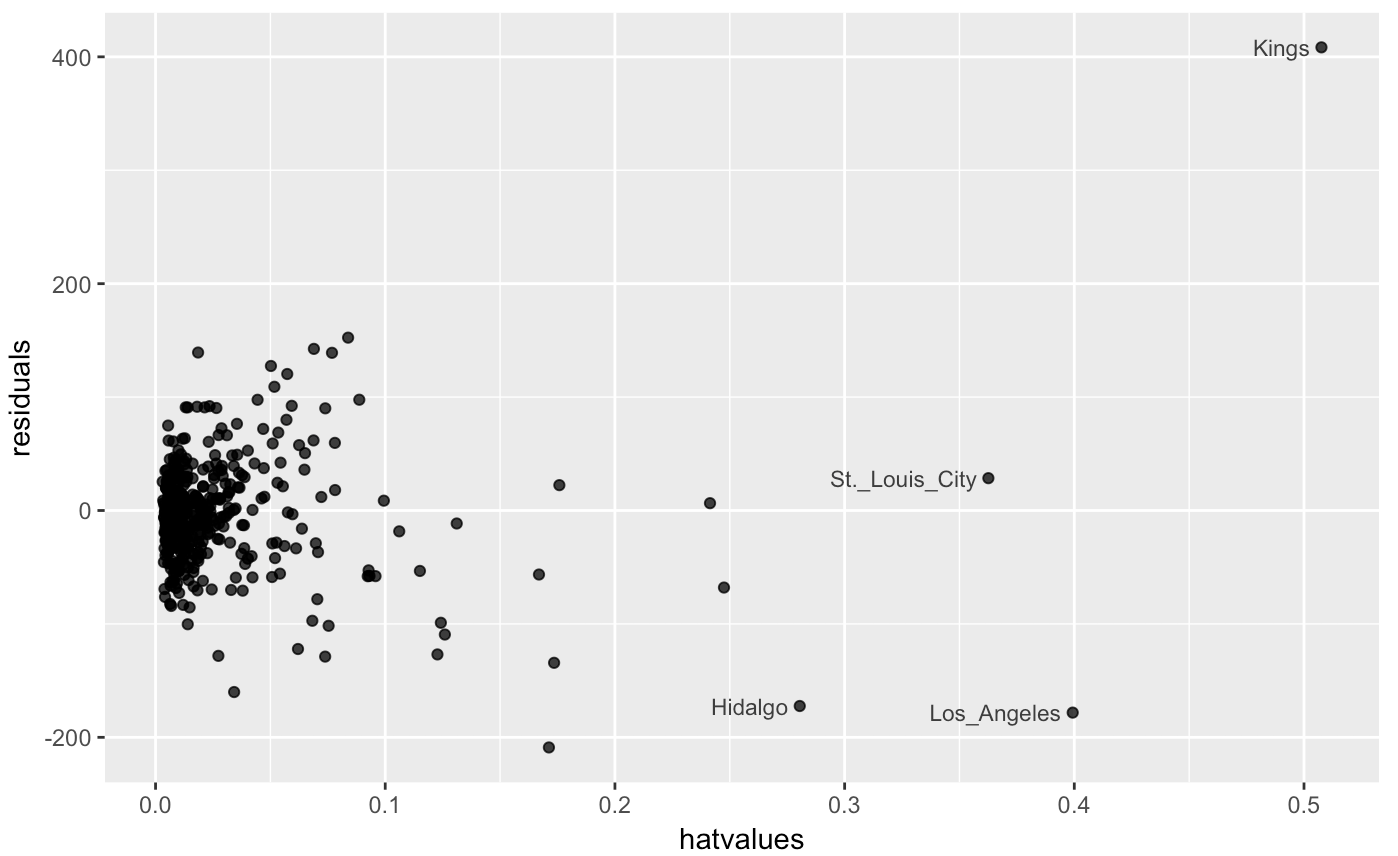
\includegraphics[scale=0.45]{hatvalue.png}
\caption{Residuals against Hatvalues} 
\end{figure}

Based on rule of thumb, hatvalues exceeding about twice the average should be considered noteworthy. Therefore in Figure 7, we find four outlier county: \textit{Kings}, \textit{St. Louis city}, \textit{Hidalgo} and \textit{Los Angeles}. We believe that our data set has some special properties: every region only appears once. So, in this problem, we should split outliers and analyze more about them.\par

As discussed in initial data exploration, further from Figure 3 and Figure 4, \textit{St. Louis city}, \textit{Hidalgo} and \textit{Los Angeles} shows the same pattern as \textit{Kings}. We find that the population density and percent of poor in these four counties is much higher than others. Therefore population density and percent of poor are important reasons for outliers and the high crime rate can also be explained.\par

After remove outliers, we refit our model and draw the residual plot:

\begin{figure}[H]
\centering
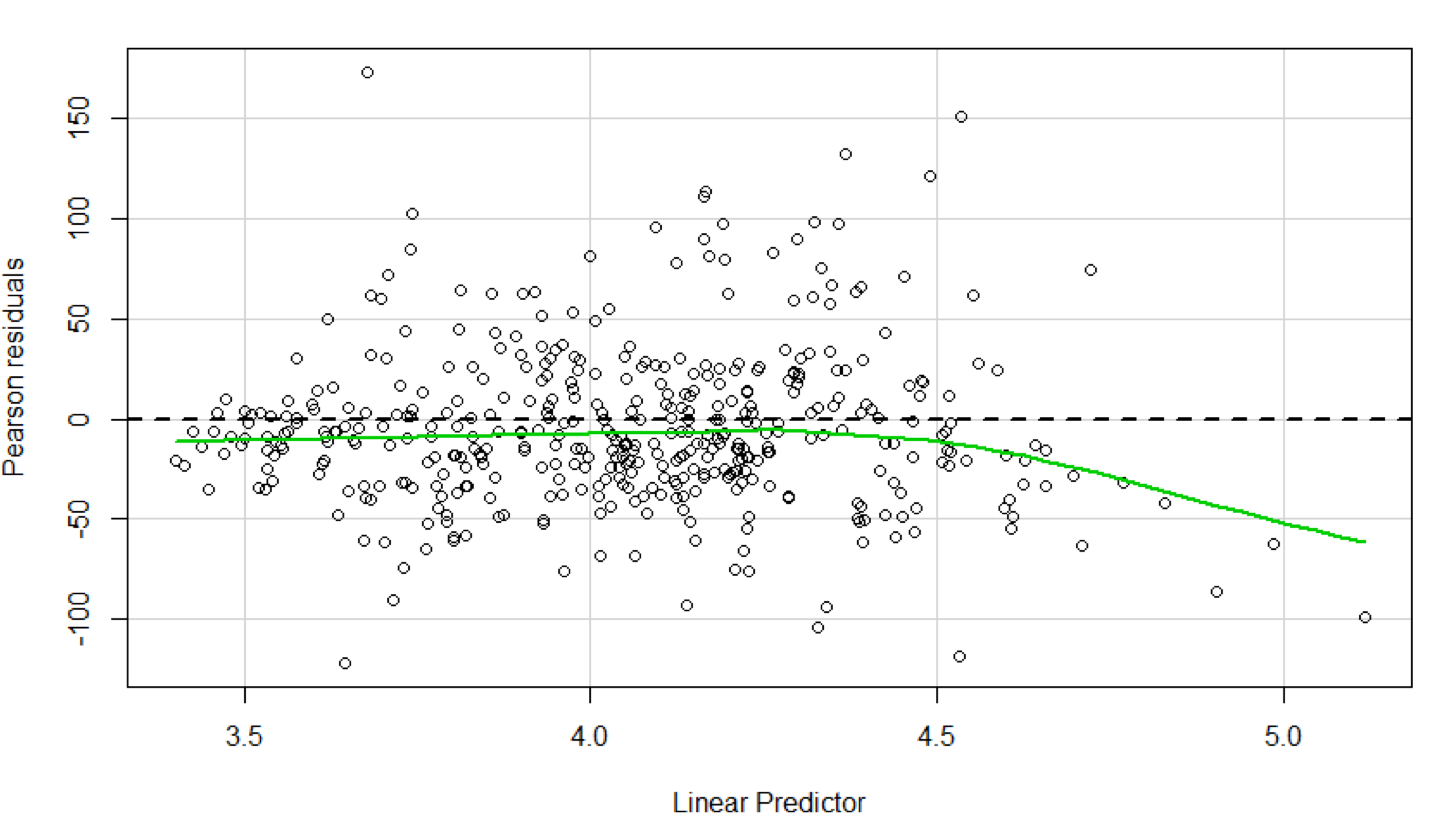
\includegraphics[scale=0.55]{residual.png}
\caption{Residual plot} 
\end{figure}

Points in the plot are randomly dispersed around the horizontal axis. Therefore our regression model is appropriate for the data. The following table gives the estimated coefficients:

\begin{table}[!hbp]
\centering
\begin{tabular}{|c|c|c|c|c|c|c|}
\hline
\hline
&percent & percent & percent & region & population & percent  \\
&poor    & income  & beds    &        & density    & physician\\
\hline
coefficients & 0.0312 & -0.00002 & 0.0286 &  $\beta\footnotemark[1]$ & 0.2106 & -0.0427 \\
\hline
exp coefficients & 1.0317 & 0.9999 & 1.0290 &  $\beta\footnotemark[2]$ & 1.2343 & 0.9582 \\
\hline
\end{tabular}

\footnotesize{$\beta$\footnotemark[1]: baseline category is region 1, estimated coefficients are $\beta_2^1 = 0.0506, \beta_3^1= 0.3462, \beta_4^1=0.3477$}\\
\leftline{~~~~~~~\footnotesize{$\beta$\footnotemark[2]: exponentiated coefficients are $\beta_2^2 = 1.0519, \beta_3^2= 1.4137, \beta_4^2=1.4158$}}
\caption{Estimated coefficient table}
\end{table}

From the analysis, we can get the interpretation of the parameter of the variable. Take percent of poor as an example, if we increase the percent below poverty level by one, the crime rate per 1000 people will times 1.0318. And decreasing the percent of hospital beds by one, the crime rate per 1000 people will divide 1.029 times. 

\subsection*{3.3 Logistic Regression}
The variable concerned is crime rate, a quantitative variable. The most weakness for quantitative variable is that it is hard to tell the crime rate of a certain number is whether severe or not. Therefore, set several threshold and convert crime rate to ordinal categorical variable. Therefore, we divide the crime rate into five categories: low, medium and high. The three categories are distinguished by two cutpoints:  60\textperthousand{} and 120\textperthousand{} correspondingly.\par

Cumulative logistic regression models are used to predict an ordinal response, and have the assumption
of proportional odds. Proportional odds means that the coefficients for each predictor category must be
consistent across all levels of the response. Therefore, a cumulative logit model is a good fit to our problem. The assumptions and conditions for the model are meeted. In this project, we assume different slopes between models and it will come out two models.\par

Before fit a cumulative logit model, we use Variance inflation factor(VIF) method to check the collinearity. The higher value of VIF, the more likely this variable is related with others. Therefore we drop the \textit{Percent bachelor’s degree} since it has high VIF(greater than 5).\par

For the model selection process, we use backward AIC to select variables. The AIC of full model using all predictor variables 864.73. After remove \textit{percent of old} \textit{percent high school graduates} and \textit{percent of physician}, we reach the lowest AIC 859.70. And this is our final logistic model.

In this part of analysis, we finally fit the final cumulative logit model that includes five predictor variables: \textit{percent of young}, \textit{percent of poor}, \textit{percent of income}, \textit{region} and \textit{population density}. The estimated coefficients are shown in Table 3.\par


\begin{table}[H]
\centering
\begin{tabular}{|c|c|c|c|c|c|c|c|}
\hline
\hline
\multicolumn{2}{|c|}{}&percent & percent & percent & percent & region & population\\
\multicolumn{2}{|c|}{}&young   & poor    & income  & beds    &        & density  \\
\hline
model&coefficients & -0.0783 & -0.1681 & -0.0001 & -0.1686 & -0.5341 & -0.00008 \\
\cline{2-8}
j=1&exp coefficients & 0.9247 &  0.8453 &  0.9999 & 0.8448 & 0.5862 &  0.9999 \\
\hline\hline
model&coefficients & 0.0028 & -0.0660 & 0.00008 & -0.7129 & -0.3486 & -0.0009 \\
\cline{2-8}
j=2&exp coefficients & 1.003 &  0.9362 &  1.000 & 0.4902 & 0.7056 &  0.9990 \\
\hline
\end{tabular}
\caption{Estimated coefficient table}
\end{table}
\par


Change of value of these explanatory variables implies a significant inluence on the crime rate. For example, when comparing odds ratio of $y=1$ and $y=2$, one unit increase of \textit{percent of poor}(i.e.percentage increases by 1\%) leads to 0.85 times of the ratio, which means a lower proportion of low crime rate to high crime rate. One unit increase of \textit{percent of young} leads to 0.92 times of the probability ratio and one unit increase of \textit{percent of beds} leads to 0.84 times of the ratio.

\section*{4 Conclusion}

The results from the three models are almost similar except some minor difference. While \textit{percent of income} is significant in logistic and poisson model but is removed in linear model. \textit{Percent of physicians} only stands out in poisson model but not significant in other two. However, the three models all generally point out the following four variables: \textit{percent of poor}, \textit{percent of hospital beds}, \textit{geographic region} and \textit{population density}. Actually, \textit{geographic region} is not changable. In the view of government, we can do nothing to it. But for citizens, based on our analysis, they can choose to live in the region that has lower crime rate, for example region in NE.\par

As for the rest variables, they can be grouped into three types: Medical support, Salary level and population density. Since the population density has significant effects on crime rate, government could decrease population density in some areas such as Kings, Los Angles, and control population density in other areas. For example, Governments could encourage some citizens to move to other regions with subsidy. However, in the real world, high population density means metropolis and high development rate in economy. Therefore, there is a tradeoff between economic development and crime rate.\par

Medical level is also a very important factors, and government should increase the investment on medical system. Government can encourage the development of health insurance, or give intervention and price control in medical costs. In our analysis, specifically, increasing the number of hospital beds is a useful method. Following this, increasing the number of hospitals and hiring more doctors and medical workers are good way to this aspect.\par

Last but not least, poverty plays an fatal role in influencing crime rate. Increasing social welfare and increasing the minimal salary level should be considered when implement policy.  Federal unemployment insurance, federal welfare programs, and medicare, all help poor and temporarily hard-pressed households make ends meet. When people's rights and lives are guaranteed, the crime rate will decrease naturally.\par


\newpage

\section*{5 Appendix}
\subsection*{5.1 Best linear model}
\begin{equation}
\begin{aligned}
crime~rate =  -23.83 &+ 0.689&\times &~perc.young \\
&+1.674&\times &~perc.poor\\
&+2.60&\times &~beds.per \\
&+9&\times &~I(region) \\
&+4.59\cdot10^{-3}&\times &~pop.density\\
\end{aligned}
\end{equation}

\subsection*{5.2 Best Poisson model}
\begin{equation}
\begin{aligned}
\frac{E(Y|X)}{\text{exposure}} &= e^{\theta X}&&\\
\theta X =  7.993
                  &+ 0.0312 &\times &perc.poor\\
                  &-0.00002 &\times &per.income\\
                  &+ 0.0286 &\times &beds.per \\
                  &+0.0506  &\times &region 2 \\
                  &+0.3462  &\times &region 3 \\
                  &+0.3477  &\times &region 4 \\
                  &+ 0.2106 &\times &pop.density\\
                  &-0.0427 &\times &perc.physician\\
\end{aligned}
\end{equation}

\subsection*{5.3 Best logistic model}
\begin{equation}
\begin{aligned}
\frac{P(Y\leq 1)}{1-P(Y\leq 1)} &= e^{\beta X}&&\\
\beta X =  7.993  &- 0.0783           &\times &perc.young \\
                  &- 0.1681           &\times &perc.poor\\
                  &- 0.0001 &\times &per.income\\
                  &- 0.1686           &\times &beds.per \\
                  &- 0.5341           &\times &I(region) \\
                  &- 0.00008 &\times &pop.density\\
\frac{P(Y\leq 2)}{1-P(Y\leq 2)} &= e^{\beta X}&&\\
\beta X =  7.401  &+ 0.0028           &\times &perc.young \\
                  &- 0.0660           &\times &perc.poor\\
                  &- 0.00008 &\times &per.income\\
                  &- 0.7129           &\times &beds.per \\
                  &- 0.3486           &\times &I(region) \\
                  &- 0.00009 &\times &pop.density\\
\end{aligned}
\end{equation}
Where $\beta_1=7.457$, $ \beta_2=10.72$, $ \beta_3 = 13.56$, and $ \beta_4=16.38$\\
Y represents the level of crime rate.





\end{document} 
